\pdfminorversion=4
\documentclass[aspectratio=169]{beamer}

\mode<presentation>
{
  \usetheme{default}
  \usecolortheme{default}
  \usefonttheme{default}
  \setbeamertemplate{navigation symbols}{}
  \setbeamertemplate{caption}[numbered]
  \setbeamertemplate{footline}[frame number]  % or "page number"
  \setbeamercolor{frametitle}{fg=white}
  \setbeamercolor{footline}{fg=black}
} 

\usepackage[english]{babel}
\usepackage[utf8x]{inputenc}
\usepackage{tikz}
\usepackage{courier}
\usepackage{array}
\usepackage{bold-extra}
\usepackage{minted}
\usepackage[thicklines]{cancel}
\usepackage{fancyvrb}

\xdefinecolor{dianablue}{rgb}{0.18,0.24,0.31}
\xdefinecolor{darkblue}{rgb}{0.1,0.1,0.7}
\xdefinecolor{darkgreen}{rgb}{0,0.5,0}
\xdefinecolor{darkgrey}{rgb}{0.35,0.35,0.35}
\xdefinecolor{darkorange}{rgb}{0.8,0.5,0}
\xdefinecolor{darkred}{rgb}{0.7,0,0}
\definecolor{darkgreen}{rgb}{0,0.6,0}
\definecolor{mauve}{rgb}{0.58,0,0.82}

\title[2018-10-15-adl-workshop-femtocode]{Making your own language: things to think about}
\author{Jim Pivarski}
\institute{Princeton University -- DIANA-HEP}
\date{October 15, 2018}

\usetikzlibrary{shapes.callouts}

\begin{document}

\logo{\pgfputat{\pgfxy(0.11, 7.4)}{\pgfbox[right,base]{\tikz{\filldraw[fill=dianablue, draw=none] (0 cm, 0 cm) rectangle (50 cm, 1 cm);}\mbox{\hspace{-8 cm}
\includegraphics[height=1 cm]{princeton-logo-long.png}
\includegraphics[height=1 cm]{diana-hep-logo-long.png}}}}}

\begin{frame}
  \titlepage
\end{frame}

\logo{\pgfputat{\pgfxy(0.11, 7.4)}{\pgfbox[right,base]{\tikz{\filldraw[fill=dianablue, draw=none] (0 cm, 0 cm) rectangle (50 cm, 1 cm);}\mbox{\hspace{-8 cm}
\includegraphics[height=1 cm]{princeton-logo.png}
\includegraphics[height=1 cm]{diana-hep-logo.png}}}}}

% Uncomment these lines for an automatically generated outline.
%\begin{frame}{Outline}
%  \tableofcontents
%\end{frame}

% START START START START START START START START START START START START START

\begin{frame}[fragile]{Domain specific languages}
\large
\vspace{0.5 cm}
Many data analysts manage to do all or most of their work with the following:

\vspace{0.5 cm}
\begin{center}
\begin{minipage}{0.85\linewidth}
\begin{minted}{sql}
SELECT expr FROM src WHERE expr GROUP BY expr
\end{minted}
\end{minipage}

\vspace{1 cm}
\uncover<2->{\Large Why do we need a full programming language?}
\end{center}
\end{frame}

\begin{frame}{Maybe it goes all the way back to the beginning?}
\vspace{0.25 cm}
\begin{center}
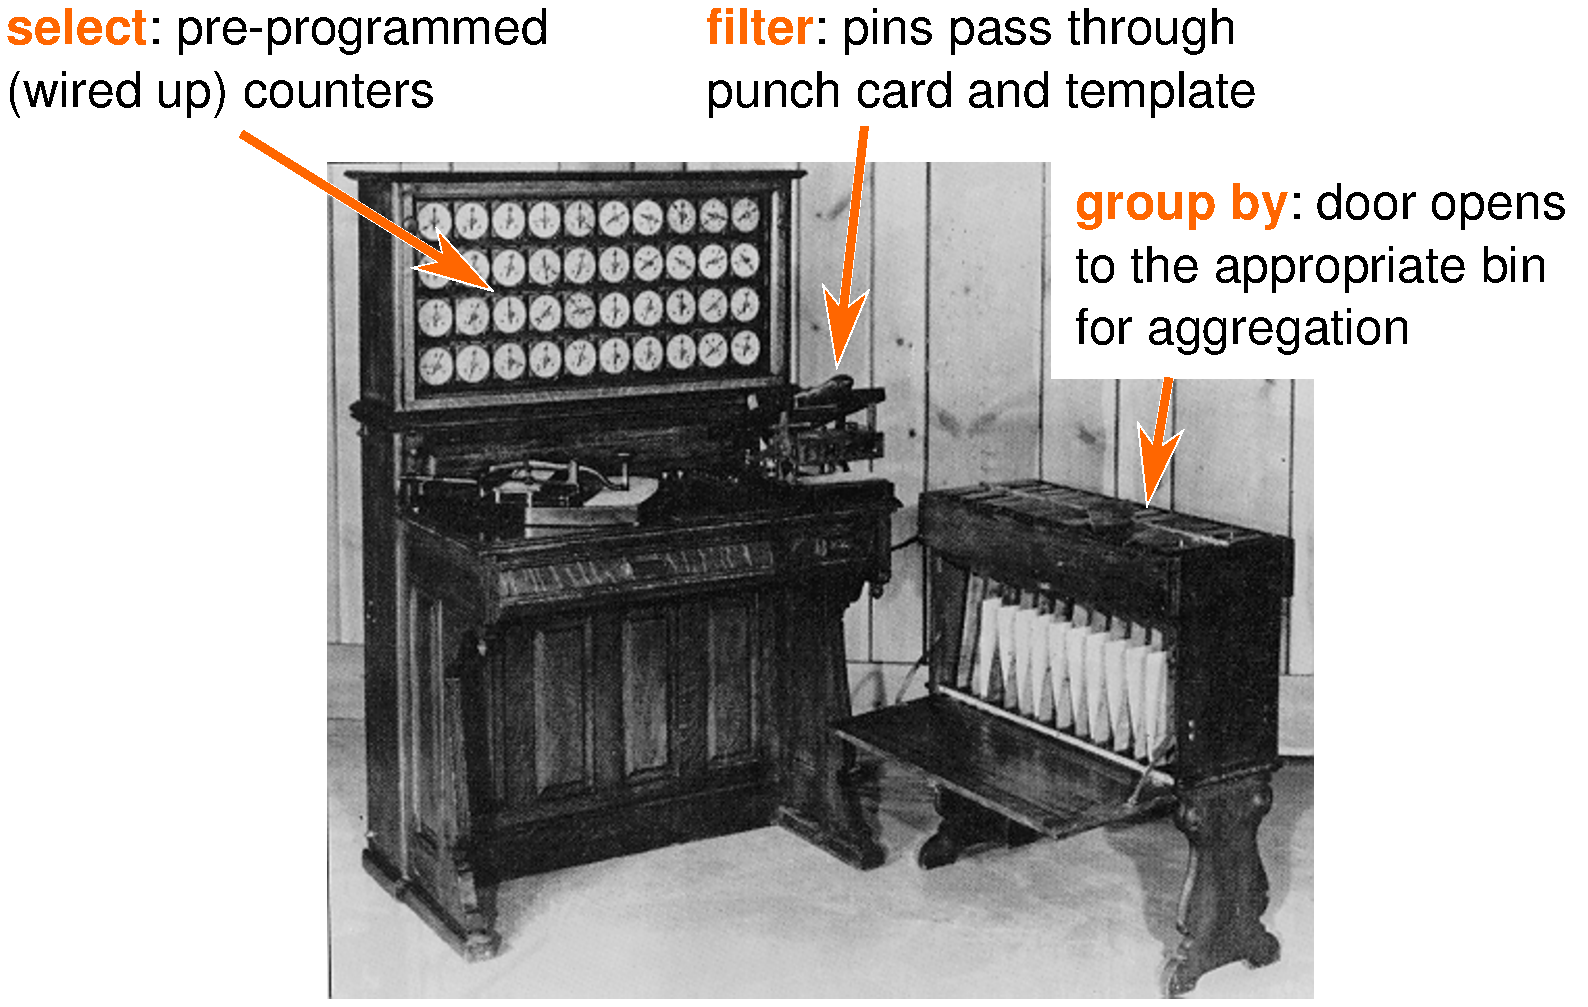
\includegraphics[width=0.83\linewidth]{hh-tabulator.pdf}
\end{center}
\end{frame}

\begin{frame}{Maybe it goes all the way back to the beginning?}
\vspace{0.5 cm}

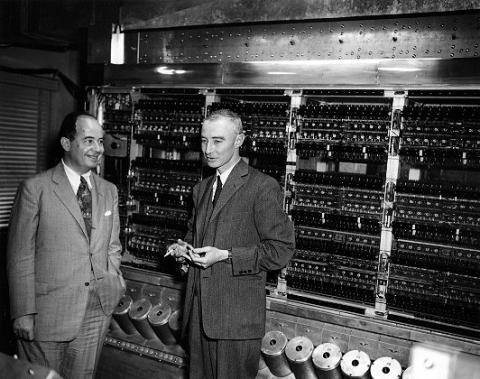
\includegraphics[height=5 cm]{neumann_oppie.jpg} 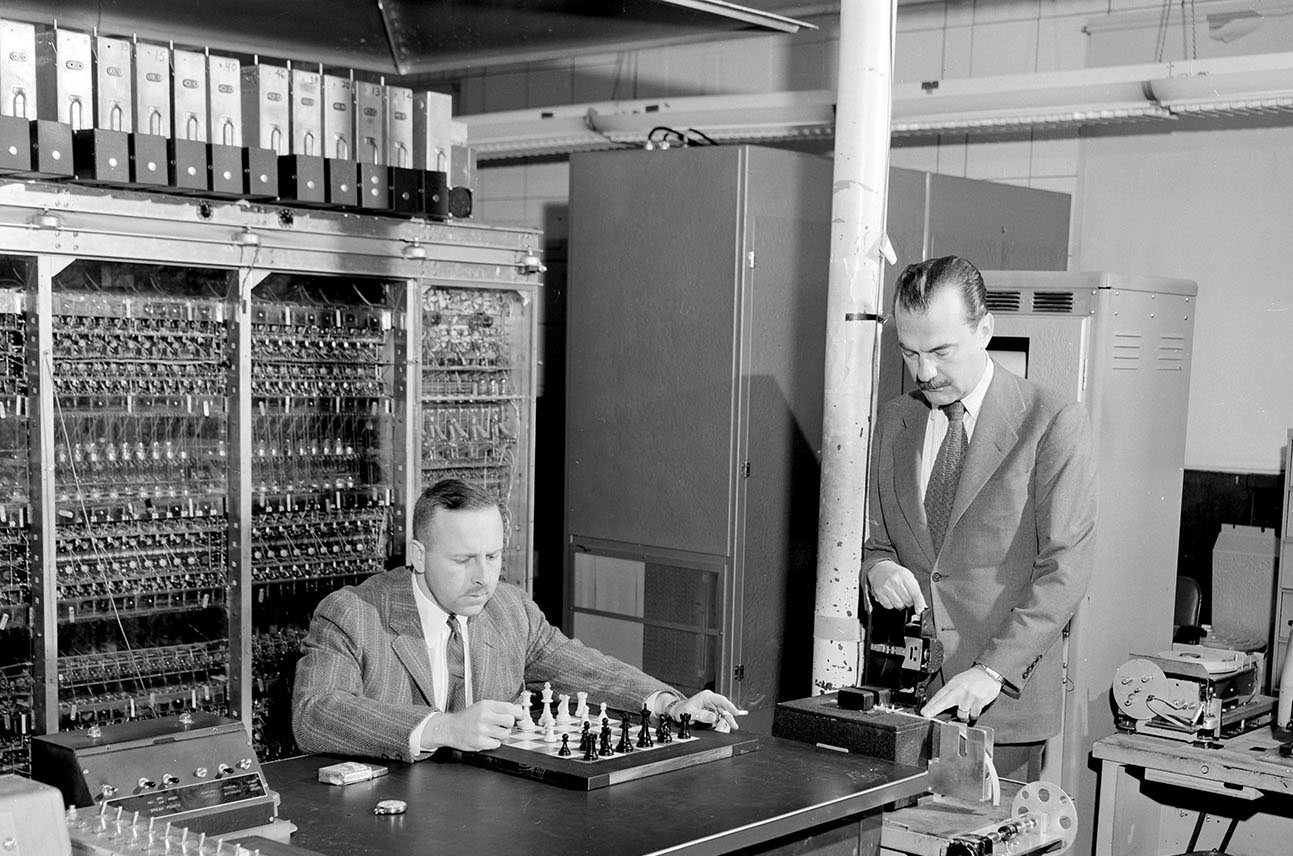
\includegraphics[height=5 cm]{metropolis.jpg}

\begin{center}
\Large {\bf M}etropolis {\bf A}nd {\bf N}eumann {\bf I}nvent {\bf A}wful {\bf C}ontraption
\end{center}
\end{frame}

\begin{frame}{Maybe it goes all the way back to the beginning?}
\large
\vspace{0.5 cm}

We're accustomed to (ab)using a complete programming environment.

\vspace{0.5 cm}
Particle physics and digital computing ``grew up together.''

\vspace{1 cm}
\uncover<2->{But what's necessary for Monte Carlo and reconstruction is often overkill for physics analysis.}
\end{frame}

\begin{frame}{Shrink-wrapping a language to the problem domain}
\large
\begin{itemize}
\item Fully featured language that makes domain-specific problems easier than general ones?
\end{itemize}

\begin{center}
\textcolor{darkorange}{\bf awk}, \textcolor{darkorange}{\bf Fortran77}, \textcolor{darkorange}{\bf Erlang}, \textcolor{darkorange}{\bf \LaTeX}, \textcolor{darkorange}{\bf PostScript}
\end{center}

\begin{itemize}
\item A limited language that can only be used on domain-specific problems?
\end{itemize}

\begin{center}
\textcolor{darkorange}{\bf SQL92}, \textcolor{darkorange}{\bf HTML4}, \textcolor{darkorange}{\bf regular expressions}, \textcolor{darkorange}{\bf configuration INI}
\end{center}
\end{frame}

\begin{frame}{Some terminology}
\large
\vspace{0.5 cm}
\begin{description}\setlength{\itemsep}{0.5 cm}
\item[Turing complete:] can do anything a Turing machine can do.

\vspace{0.25 cm}
{\normalsize For example, conditional branching $+$ ability to store and retrieve any number of variables.}

\item[Declarative:] order of expressions does not imply any order of computations.

\vspace{0.25 cm}
{\normalsize For example, SQL SELECT may be computed before or after SQL WHERE. The first HTML element is drawn {\it above} the second, but not necessarily {\it before}.}

\item[Functional:] computations are defined in terms of functions that accept or return functions, usually with immutable data.

\vspace{0.25 cm}
{\normalsize For example, \small\mintinline{scala}{data.map(ev => ev.muons.maxby(mu => mu.pt))}\normalsize .}
\end{description}
\end{frame}

\begin{frame}[fragile]{``Declarative'' is being abused}
\small
\vspace{0.25 cm}
\begin{minted}{python}
def infinite_loop():
    return infinite_loop()

def simple_boolean():
    return False

infinite_loop() and simple_boolean()    # runs forever
simple_boolean() and infinite_loop()    # returns False
\end{minted}

\normalsize
\vspace{0.25 cm}
A truly declarative language would be insensitive to order and either always run forever or always short-circuit the boolean logic.

\vspace{0.5 cm}
It's hard for a declarative language to be Turing complete.

\vspace{0.5 cm}
When physicists say ``declarative,'' they usually mean ``functional.'' 
\end{frame}



\end{document}
